\question[15]  El diagrama muestra un triángulo rectángulo y tres cuadrados.
El área del cuadrado más grande es 55 unidades$^2$, como se muestra en la figura \ref{fig:area11}.
\begin{figure}[H]
    \begin{center}
        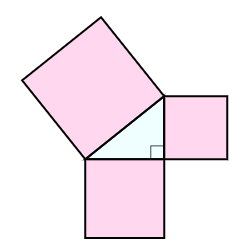
\includegraphics[width=0.4\textwidth]{../images/area11.png}
    \end{center}
    \caption{}
    \label{fig:area11}
\end{figure}

\begin{parts}
    \part \textbf{¿Cuáles pueden ser las áreas de los cuadrados más pequeños?}
    \begin{checkboxes}
        \choice 12 y 43
        \choice 14 y 40
        \choice 16 y 37
        \choice 44 y 11
        \choice 5 y 11
        \choice 20 y 25
        \choice 10 y 45
        \choice 16 y 39
    \end{checkboxes}
\end{parts}